\documentclass{beamer}
\usetheme{Madrid}

\usepackage{graphicx}
\usepackage{bibentry}
\usepackage[utf8]{inputenc}
\usepackage[T1]{fontenc}


\date{\today}
\title{Červeno-čierny strom \\ 5. projekt, ITY}
\author{Katarína Mečiarová}

%struktura
\begin{document}

    \frame[plain]{\titlepage}

%2
    \begin{frame}
        \frametitle{Motivácia}
        \begin{itemize}
            \item \textbf{Algoritmy} sú jedným zo \textbf{základných prvkov spracovania informácií}
            \vfill
            \item Čo je to \textbf{červeno-čierny strom}?
            \vspace{10pt}
            \\ \footnotesize{Od vzniku, cez praktické využitie až do končín teórie}
        \end{itemize}
    \end{frame}

%3
    \begin{frame}
        \frametitle{"\ldots the rest is history"}
        \begin{columns}
            \column{0.5\textwidth}
            \begin{itemize}
                \item Kto? \textbf{Rudolf Bayer}
                \vspace{5pt} \\ \footnotesize{symetrický binární B-strom} \vspace{10pt} \\
                Leo J. Guibase, Robert Sedgewick
                \vspace{10pt} \\
                \item \normalsize{Kedy}? \textbf{1972}, \\ \vspace{5pt}
                {\footnotesize{premenované 1978, \ldots 1993, 1999}}  \vspace{15pt}
                \item Ako? \footnotesize{To si rozoberieme na drobné v nasledujúcom slajde}
            \end{itemize}
            \column{0.5\textwidth}
            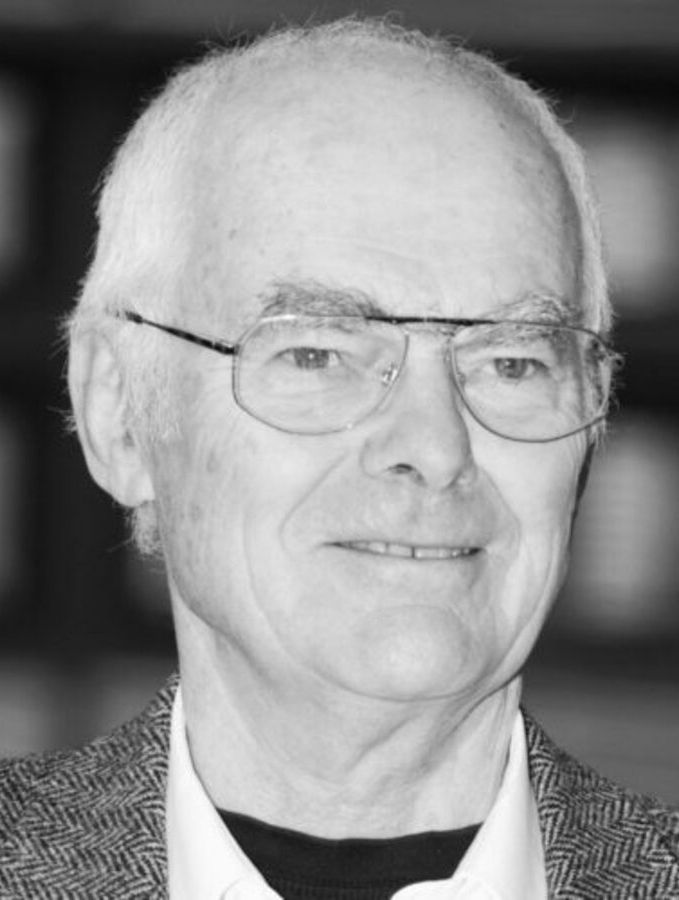
\includegraphics[width=150pt]{bayer}
        \end{columns}
    \end{frame}

%4
    \begin{frame}
        \frametitle{"\ldots the rest is history"}

        \textbf{1972}
        \\ {\footnotesize{R. Bayer prišiel s novou dátovou štruktúrou, tvoriacou "dokonale vyrovnané stromy"}} \\

        \vspace{10pt}
        \textbf{1978}
        \\ {\footnotesize{Guibas a Sedgewick spomenuli štruktúru pod menom "červeno-čierny strom" \\
        význam výberu červenej farby bol čisto pragmatický}} \\

        \vspace{10pt}
        \textbf{1993}
        \\ {\footnotesize{\textbf{Arne Andersson} predstavil svetu "LL strom" - zjednodušenie a vyrovnanie}}

        \vspace{10pt}
        \textbf{1999}
        \\ {\footnotesize{\textbf{Chris Okasaki} objavil nový spôsob a tak pracoval len so 4 nevyrovnanými prípadmi}}



        \begin{center}
            \ldots \\
            Čo s tým?
        \end{center}
    \end{frame}

%5
    \begin{frame}
        \frametitle{Využitie v praxi}
        \begin{columns}
            \column{0.5\textwidth}
            \begin{itemize}
                \item funkcionálne programovanie
                \item real-time procesy (RTC)
                \item geometrické algoritmy
                \vspace{20pt}
                \item asociatívne reťazce
                \item množiny
                \item slovníky
            \end{itemize}
            \column{0.5\textwidth}
            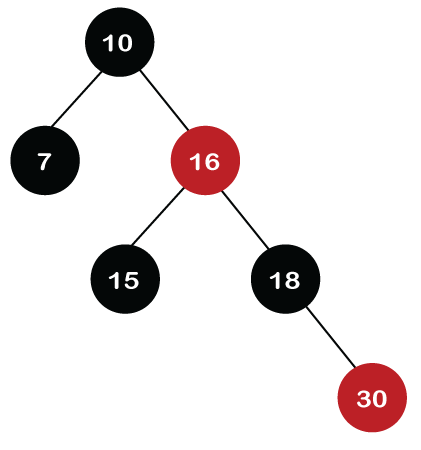
\includegraphics[width=150pt]{rbt17}
        \end{columns}
    \end{frame}

%6
    \begin{frame}
        \frametitle{Definícia štruktúry}
        \begin{enumerate}
            \item Každý vrchol je buď čierny alebo červený.
            \item Koreň, materský vrchol je čierny.
            \item Ak je vrchol červený, obe jeho deti sú čierne.\\
            Žiadny červený vrchol nemá žiadne červené dieťa.
            \item Každá cesta z (akéhokoľvek) vrcholu do (akéhokoľvek) listu má rovnaký počet čiernych vrcholov.
        \end{enumerate}
        \vspace{20pt}
        Teda ak vrchol \textbf{N} má presne \textbf{1 dieťa}, tak to dieťa \textbf{musí byť červené}. \\
        \vspace{5pt}
        {\footnotesize{\textbf{Ak by bolo dieťa čierne, jeho NIL potomkovia by sa nachádzali v inej (čiernej) hĺbke ako NIL potomok N, čím by sa porušila požiadavka 4.}}}

        \vspace{15pt}
        \centering{Zapisujeme pomocou Landauovej notácie.}
    \end{frame}

%7
    \begin{frame}
        \frametitle{Základné operácie}
        \begin{itemize}
            \item pridať vrchol/list
            \item odstrániť
            \item preoznačiť {\footnotesize{(zmena farby vrcholu)}}
            \item zlúčenie stromov
            \item rozdelenie stromu
            \item rotácie
            \begin{itemize}
                \item pravá
                \item ľavá
            \end{itemize}
        \end{itemize}
    \end{frame}

%8
    \begin{frame}
        \frametitle{Pseudokód pridatia prvku}
        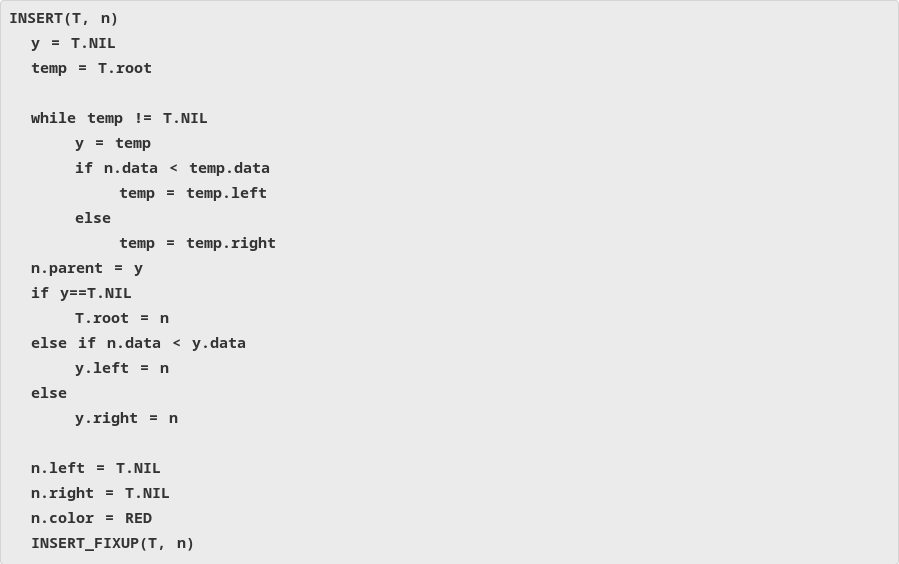
\includegraphics[width=\textwidth]{in}
    \end{frame}

%9
    \begin{frame}
        \frametitle{Pseudokód rotácie}
        \begin{columns}
            \column{0.65\textwidth}
            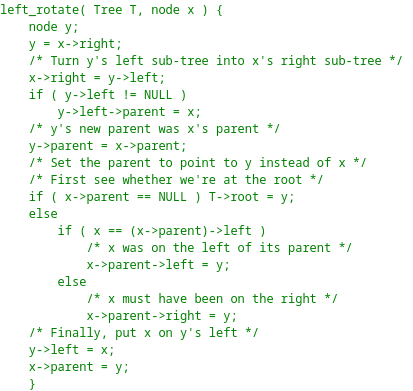
\includegraphics[width=\textwidth]{code}
            \column{0.35\textwidth}
            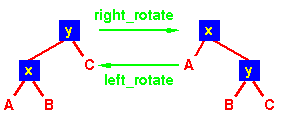
\includegraphics[width=\textwidth]{rot}
        \end{columns}
    \end{frame}

%10
    \begin{frame}
        \frametitle{Odvíjajúce sa}
        \begin{itemize}
            \item AVL strom
            \item AA strom
            \item B strom, B+ strom, \ldots
            \item T strom
            \item WAVL strom
            \item Splay strom
            \item Scapegoat strom
        \end{itemize}
    \end{frame}

%11
    \begin{frame}
        \frametitle{Ďakujem za Vašu pozornosť}
        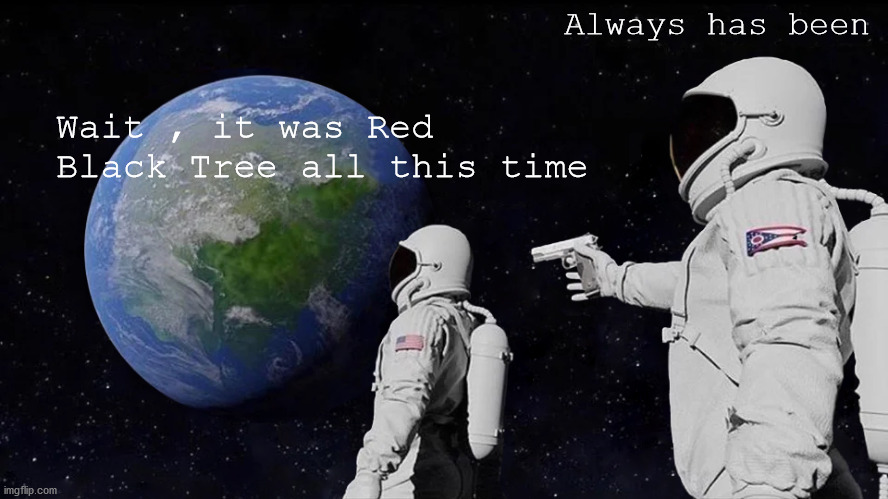
\includegraphics[width=\textwidth]{meme}
    \end{frame}

%12
    \begin{frame}
        \frametitle{Zdroje}~\nocite{*}
        \bibliographystyle{czechiso}
        \bibliography{references}
    \end{frame}

\end{document}